\section{Introduction}
Une \emph{anomalie}, du grec $\alpha \nu \omega \mu \alpha \lambda \iota \alpha $, aspérité, irrégularité, "non-semblable" (an-homalos), désigne un écart par rapport à une certaine normalité, par rapport à un comportement attendu.
On appelle \emph {anomalie} l'objet qui induit cet espace, l'observation qui s'écarte de la normalité.
%
Dans beaucoup de domaines, la situation suivante se présente: un expert cherche à prédire un phénomène sur la base d'observations antérieures. Le cas le plus fondamental est lorsque l'on veut prédire certaines caractéristiques binaires d'observations nouvelles, compte tenu des précédentes. Par exemple, on peut penser à un médecin voulant prédire si un nouveau patient présente ou non une certaine pathologie, en utilisant les données des patients précédents (comme l'âge, l'histoire, le sexe, la pression artérielle) associées à leur véritable \textbf{étiquette/label}: avoir ou non la pathologie en question. Ce cas est un exemple de \emph {classification binaire}, où le médecin cherche à trouver une règle pour \textbf {prédire} l'étiquette d'un nouveau patient (ce dernier étant caractérisé par son dossier médical, contenant toutes les mesures qui lui ont été faites). Cette règle est appelée un \emph{classifieur} et doit être construite, \emph{apprise}, sur des dossiers médicaux précédents. % (À savoir les enregistrements associés à leurs étiquettes).
Intuitivement, le classificateur prédit le même diagnostic pour des dossiers médicaux similaires, dans un sens qui doit être appris avec précision.

On peut distinguer deux cas. Si les étiquettes des patients antérieurs sont connues (porteur ou non de la pathologie), on dit que la tâche de classification est \textbf {supervisée}. Si les étiquettes de ces données d'entrainement sont inconnues, la classification est dite \textbf {non-supervisée}. Suivant notre exemple, le médecin doit trouver deux formes (ou cluster) distinctes dans les données, correspondant aux deux étiquettes, "en bonne santé" - "malade", formes qui contiennent chacune des dossiers de patients similaires.

La détection d'anomalies survient lorsqu'une étiquette est fortement sous-représentée dans les données d'entrainement, par exemple si très peu de patients ont la pathologie dans les données d'entrainement.
Ainsi, la \textbf{détection d'anomalies supervisée} se résume à la classification supervisée de classes fortement déséquilibrées.
En ce qui concerne la \textbf {détection d'anomalies non supervisée} (également appelée simplement \textbf{détection d'outliers}), elle suppose généralement que la base de données a un modèle "normal" caché, et les anomalies sont des observations qui s'écartent de ce modèle. Le médecin veut trouver des dossiers médicaux qui s'écartent de la grande majorité de ceux de ses patients précédents.
%
Sa tâche est en quelque sorte simplifiée s'il sait que tous ses patients antérieurs sont en bonne santé: il est plus facile pour lui d'apprendre le modèle "normal", c'est-à-dire le dossier médical typique d'un patient en bonne santé, à confronté avec les dossiers médicaux de ses nouveaux patients. Ce cadre est celui de la \textbf {détection de nouveauté} -- également appelé classification à une classe ou détection d'anomalies semi-supervisées: les données d'entraînement ne contiennent que des instances normales.

Ce résumé introductif est organisé de la façon suivante.
Section~\ref{resume_fr:scoring_function}, la détection d'anomalies est formellement introduite, ainsi que la notion de fonction de score.
Deux critères sur la qualité d'une fonction de score sont ensuite présentés section~\ref{resume_fr:scoring}.
La section~\ref{resume_fr:extreme} se concentre sur la théorie des valeurs extrêmes (TVE) pour gagner en précision sur les régions extrêmes. Après avoir introduit la STDF (stable tail deviation function) représentant la structure de dépendance des événements rares (section~\ref{resume_fr:stdf}), on montre que la théorie des extrêmes multivariées peut être utile pour produire des fonctions de score précise sur les régions de faible probabilité (section~\ref{resume_fr:sec:JMVA}).
La section~\ref{resume_fr:sec:heuristic} regroupe deux contributions de nature heuristique portant d'une part sur l'évaluation / la sélection d'algorithmes de détection d'anomalies non supervisés (section~\ref{resume_fr:evaluation}) et d'autre part sur l'extension des forêts aléatoires à la classification à une classe (section~\ref{resume_fr:ocrf}). La section~\ref{resume_fr:sec:impl} présente les contributions relatives à la librairie open-source scikit-learn. La section~\ref{resume_fr:intro:concl} énumère les productions scientifiques et conclut.


\paragraph{Notations.}

A travers ce document, $\mathbb{N}$ désigne l'ensemble des entiers naturels, $\mathbb{R}$ and $\mathbb{R}_+$ désignent respectivement l'ensemble des nombres réels et celui des nombres réels positifs. Les ensembles  sont généralement écrit en lettre calligraphiques comme $\mathcal{G}$, et $|\mathcal{G}|$ désigne le nombre d'éléments dans $\mathcal{G}$. 

Les vecteurs sont écrits en minuscules et en gras. Pour un vecteur $\mathbf{x}\in\mathbb{R}^d$ et $i\in \{1,\dots,d\}$, $x_i$ désigne la $i^{eme}$ composante de $\mathbf{x}$. Le produit scalaire entre deux vecteurs est noté $\innerp{\cdot,\cdot}$. $\|\cdot\|$ désigne une norme arbitraire (sur des vecteurs ou sur des matrices) et $\|\cdot\|_p$ la norme $L_p$.

Au long de cette thèse, $\PP[A]$ représente la probabilité de l'évènement $A\in \Omega$, l'espace de probabilité sous-jacent étant $(\Omega, \mathcal{F}, \PP)$. Nous utilisons la notation $\mathbb{E}[X]$ pour indiquer l'espérance de la variable aléatoire $X$. La notation $X \overset{d}{=} Y$ signifie que $X$ et $Y$ sont égales en distribution et $X_n \overset{d}{\to} Y$ signifie que $(X_n)$ converge vers $Y$ en distribution. Nous utilisons souvent l'abréviation $\mb X_{1:n}$ pour désigner un échantillon \iid~$(\mb X_1,\ldots,\mb X_n)$.

% Les notations sont résumées \tref{resume_fr:tab:notations}.

% \begin{table}[!ht]
% \begin{center}
% \begin{footnotesize}
% \begin{tabular}{lp{1cm}l}
% \toprule
% \textbf{Notation} && \textbf{Description}\\
% \midrule
% $\cdf$ && cumulative distribution function\\
% $\rv$ && random variable\\
% $\mathbb{R}$ && Set of real numbers\\
% $\mathbb{R}_+$ && Set of nonnegative real numbers\\
% $\mathbb{R}^d$ && Set of $d$-dimensional real-valued vectors\\
% $\leb(\cdot)$ && Lebesgue measure on $\mathbb{R}$ or $\mathbb{R}^d$\\
% $(\cdot)_+$ && positive part\\
% $\vee$ && maximum operator\\
% $\wedge$ && minimum operator\\
% %$\mathbb{R}^{c\times d}$ && Set of $c\times d$ real-valued matrices\\
% $\mathbb{N}$ && Set of natural numbers, i.e., $\{0,1,\dots\}$\\
% %$\mathbb{S}^{d}_+$ && Cone of symmetric PSD $d\times d$ real-valued matrices\\
% %$[k]$ && The set $\{1,2,\dots,k\}$\\
% $\mathcal{G}$ && An arbitrary set\\
% $|\mathcal{G}|$ && Number of elements in $\mathcal{G}$\\
% %$\mathcal{G}^m$ && A set of $m$ elements from $\mathcal{S}$\\
% %$\mathcal{X}$ && Input space\\
% %$\mathcal{Y}$ && Output space\\
% %$z=(x,y)\in\mathcal{X}\times\mathcal{Y}$ && An arbitrary labeled instance\\
% $\mathbf{x}$ && An arbitrary vector\\
% $\mb x < \mb y$ && component-wise vector comparison\\
% $\mb m$ (for $m \in \rset$) && vector $(m,\ldots,m)$\\
% $\mb x < m$ && means $\mb x < \mb m$\\
% $x_j$ && The $j^{th}$ component of $\mathbf{x}$\\
% $\delta_{\mb a}$ && Dirac mass at point $a \in \mathbb{R}^d$\\
% $\lfloor \cdot \rfloor$ && integer part\\
% $\innerp{\cdot,\cdot}$ && Inner product between vectors\\
% %$[\cdot]_+$ && Hinge function\\
% %$\mathbf{M}$ && An arbitrary matrix\\
% %$\mathbf{I}$ && The identity matrix\\
% %$M_{i,j}$ && Entry at row $i$ and column $j$ of matrix $\mathbf{M}$\\
% $\|\cdot\|$ && An arbitrary norm\\
% $\|\cdot\|_p$ && $L_p$ norm\\
% %$\mathsf{x}$ && An arbitrary string\\
% %$|\mathsf{x}|$ && Length of string $\mathsf{x}$\\
% %$\mathsf{x_i},\mathsf{x_{i,j}}$ && $j^{th}$ symbol of $\mathsf{x}$ and $\mathsf{x_i}$\\
% %$x\sim P$ && $x$ is drawn i.i.d. from probability distribution $P$\\
% $A\Delta B$ && symmetric difference between sets $A$ and $B$ \\
% $(\Omega, \mathcal{F}, \PP)$ && Underlying probability space\\
% $\mathcal{S}$ && functions $s: \mathbb{R}^d \rightarrow \mathbb{R}_+ $ integrable \wrt~ Lebesgue measure (scoring functions)\\
% $\overset{d}{\to}$ && Weak convergence of probability measures or \rv\\
% $\mathbf{X}$ && A \rv~with values in $\mathbb{R}^d$\\
% $\mathds{1}_{\mathcal{E}}$ && indicator function event $\mathcal{E}$\\
% $Y_{(1)} \le \ldots\le Y_{(n)}$ && order statistics of $Y_1,\ldots,Y_n$\\
% $\mb X_{1:n}$ && An \iid~sample $(\mb X_1,\ldots,\mb X_n)$\\
% $\PP[\cdot]$ && Probability of event\\
% $\EE[\cdot]$ && Expectation of random variable\\
% $\Var[\cdot]$ && Variance of random variable\\

% \bottomrule
% \end{tabular}
% \end{footnotesize}
% \caption[Résumé des notations]{Summary of notation.}
% \label{resume_fr:tab:notations}
% \end{center}
% \end{table}


\section{Détection d'anomalies, ranking d'anomalies et fonctions de scores}
\label{resume_fr:scoring_function}
D'un point de vue probabiliste, il existe différentes façons de modéliser les comportements normaux et anormaux, ce qui conduit à différentes méthodologies. Un modèle probabiliste naturel consiste à supposer deux processus de génération différents pour les données normales et anormales. Les données normales (resp. données anormales) sont générées selon une distribution $F$ (respectivement $G$). La distribution sous-jacente générale est alors un mélange de $F$ et $G$. L'objectif est de déterminer si une nouvelle observation $ \mb x $ a été générée à partir de $ F $ ou de $ G $. Le meilleur moyen de résoudre théoriquement ce problème est le test du rapport de vraisemblances, également appelé test de Neyman-Pearson. Si $ (\ud F / \ud G) (\mb x)> t $ avec un certain seuil $ t> 0 $, alors $ \mb x $ a été généré selon $ F $. Sinon, $ \mb x $ a été généré selon $G$. Cela revient à estimer l'\emph{ensemble de niveau de densité} $ \{\mb x, (\ud F / \ud G) (\mb x)> t \} $ \citep{Scholkopf2001, Steinwart2005, Scott2006, VertVert}.
%
Comme les anomalies sont très rares, leur structure ne peut être observée dans les données, en particulier leur distribution $ G $.
%
Il est courant et commode de remplacer $ G $ dans le problème ci-dessus par la mesure de Lebesgue, de sorte qu'il se résume à l'estimation du niveau de densité de $ F $.
\citep{Scholkopf2001, Scott2006, VertVert}.

Cela revient à supposer que les anomalies sont uniformément réparties sur le support de la distribution normale. % \Citep {Steinwart2005, Blanchard2010}.
Cette hypothèse est donc implicitement faite par une majorité d'ouvrages sur la détection de nouveauté / classification à une classe.
%
Nous observons les données dans $ \rset ^ d $ à partir de la classe normale seulement, avec une distribution sous-jacente $ F $ et avec une densité $ f: \rset ^ d \to \rset $.
% Les données anormales sont présumées être dans la queue de $ F $.
Le but est d'identifier les caractéristiques de cette classe normale, telles que son support $ \{\mb x, f (\mb x)> 0 \} $ ou un certain niveau de densité fixé $ \{\mb x, f (\mb x )> T \} $ avec $ t> 0 $ près de $ 0 $.

La détection d'anomalies non supervisée est souvent considérée comme un problème de classification à une classe, où les données d'entraînement sont polluées par quelques éléments de la classe anormale: elle fait appel à des algorithmes à une classe \emph{robustes} aux anomalies.

%This way of modeling appeals for \emph{density level set estimation} analysis.

Une idée naturelle pour estimer les ensembles de niveau de densité est de calculer une estimation de la densité et de considérer les ensembles de niveau associés \citep{Tsybakov1997, Cuevas1997, Baillo2001, Baillo2003, Cadre2006, Rigollet2009, Mason2009}.
La densité est généralement estimée à l'aide d'un estimateur à noyau non paramétrique ou d'un estimateur de maximum de vraisemblance à partir d'une famille paramétrique de fonctions. Mais ces méthodes ne s'adaptent pas bien à la  grande dimension. D'une certaine manière, ces méthodes cherchent à capturer plus d'information que nécessaire pour la tâche d'estimation d'ensemble de niveau, comme les propriétés locales de la densité qui sont inutiles pour cette tache. En effet, il s'avère que pour toute transformation croissante $ T $, les ensembles de niveau de $ T \circ f $ sont exactement ceux de $ f $. Ainsi, il suffit d'estimer n'importe quel représentant de la classe des transformées croissantes de $ f $, pour obtenir des estimés d'ensemble de niveau. Intuitivement, il suffit d'estimer le pré-ordre (le \emph {scoring}) induit par $ f $ sur $ \rset ^ d $. Définissons une \emph {fonction de score} comme toute fonction mesurable $ s:~ \rset ^ d \to \rset _ + $ intégrable par rapport à la mesure de Lebesgue $ \leb (.) $ et $ \S $ l'espace de toutes les fonctions de score.
Toute fonction de score définit un pré-ordre sur $ \rset ^ d $ et donc un classement sur un ensemble de nouvelles observations. Ce classement peut être interprété comme un degré d'anormalité, plus $ s (x) $ est petit, plus $ x $ est normal. Notons que la plupart des algorithmes de détection d'anomalies renvoient plus qu'une étiquette binaire, normale / anormale. Ils renvoient une fonction de score, qui peut être convertie en prédiction binaire, généralement en imposant un seuil basé sur sa distribution statistique.


Supposons que nous voulons apprendre une fonction de score $ s $ dont le pré-ordre induit est "proche" de celui de $f$, ou de manière équivalente dont les ensembles de niveau induits sont proches de ceux de $ f $. Le problème est de transformer cette notion de proximité en critère $ \crit $, les fonctions de score optimales $ s ^ * $ étant alors définies comme celles qui optimisent $ \crit $. Dans le cadre de l'estimation de la densité, la différence uniforme $ \| f - \hat f \|_\infty $ est un critère commun pour évaluer la qualité de l'estimation. Nous aimerions un critère similaire, mais qui est invariant par transformé croissante de $ \hat f $. En d'autres termes, le critère doit être défini de telle sorte que la collection d'ensemble de niveau d'une fonction de score optimale $ s ^ * (x) $ coïncide avec celle relative à $ f $, et toute transformation croissante de la densité devrait être optimale au sens de $ \crit $.
Plus formellement, nous allons considérer $ \crit ^ {\Phi} (s) = \| \Phi(s)  - \Phi (f) \| $ (au lieu de $ \| s - f \| $) 
avec $ \Phi: \mathbb {R} \to \mathbb {R} _ + $ vérifiant $ \Phi (T \circ s) = \Phi (s) $ pour toute fonction de score $ s $ et transformation croissante $ T $. Ici $ \Phi (s) $ désigne soit la courbe masse-volume $ MV_s $ de $ s $, soit sa courbe en excès-masse $ EM_s $, définies dans la section suivante.

Ce critère qui mesure la qualité d'une fonction de score est alors un outil pour construire / apprendre une bonne fonction de score.
Selon le paradigme de la minimisation du risque empirique, une fonction de score est construite en optimisant une version empirique $ \crit_n (s) $ du critère sur un ensemble adéquat de fonctions de score $ \S_0 $ de complexité contrôlée (par exemple une classe de dimension {\sc VC} finie).

La section suivante décrit deux critères fonctionnels au vue de la nature globale du problème, tout comme les courbes \roc~(\emph{Receiver Operating Characteristic}) et PR (\emph {Precision-Recall}), et qui sont admissibles par rapport aux exigences énumérées ci-dessus. Ces critères fonctionnels étendent en quelque sorte le concept de la courbe $ \roc $ au cadre non-supervisé.

\begin{remarque}{\bf Terminologie: détection d'anomalies, ranking d'anomalies.\\}
À proprement parler, les critères que nous recherchons sont des critères de \emph{ranking} d'anomalies, de la même manière que la courbe ROC est essentiellement un critère de \emph{ranking} bipartite.
%
En pratique comme mentionné ci-dessus, tous les algorithmes de détection d'anomalies sont candidats à la tâche de ranking d'anomalie. Ils produisent tous une fonction de score, même ceux qui traitent à l'origine du cadre de "classification des anomalies", c'est à dire cherchent à être optimal sur un seul ensemble de niveau ou pour un taux de faux positifs fixe.
%
Dans la littérature, la terminologie "détection d'anomalies" est largement utilisée, au lieu de la terminologie plus précise de "ranking d'anomalies". Par exemple, \cite{Liu2008} écrit "\emph{Le but de la détection d'anomalies est de fournir un ranking qui reflète le degré d'anomalie}".
%
Dans le cadre de ce travail, nous optons de même pour la convention que la détection d'anomalies se réfère au ranking d'anomalies: si les labels sont disponibles pour l'étape d'évaluation, l'objectif est de maximiser l'aire sous la courbe ROC. Si aucune donnée labelisée n'est disponible, l'objectif est de maximiser les critères non-supervisées définis dans la section suivante.

\end{remarque}


\section{M-estimation et critères de performance pour les fonctions de scores}
\label{resume_fr:scoring}
Cette section est basée sur le travail \cite{AISTAT15}. Nous fournissons un bref aperçu du critère de la courbe masse-volume introduit dans \cite{CLEM13}, qui est basé sur la notion d'ensembles de volume minimum. Nous exposons ensuite les principaux inconvénients de cette approche et proposons un autre critère, la courbe d'excès de masse.

\subsection{Ensembles à volume minimal}
\label{resume_fr:mv-set}

La notion d'ensemble de volume minimal (\cite{Polonik97, Einmahl1992}) a été introduite pour décrire des régions où une variable aléatoire multivariée $\mb X \in \rset^d$  se trouve avec très grande ou très petite probabilité. Soit $\alpha \in (0,1)$, un ensemble de volume minimal $\Gamma^*_{\alpha}$ de masse au moins $\alpha $ est une solution du problème de minimisation sous contrainte

\begin{equation}\label{resume_fr:eq:MV}\min_{\Gamma~ \text{borelien}} ~\leb(\Gamma) \mbox{~tel que~} \mathbb{P}(\mb X \in \Gamma) \ge \alpha,
\end{equation}

le minimum étant pris sur tous les sous-ensembles mesurables $ \Gamma $ de $ \rset^d $.
On peut montrer que chaque niveau de densité est un ensemble de volume minimal pour une certaine masse et que la réciproque est vraie si la densité n'a pas de partie plate.
Dans le reste de cette section, on suppose que $F$ a une densité $ f(x) $ par rapport à la mesure de Lebesgue sur $ \rset^d $ satisfaisant les hypothèses suivantes:

\noindent $\mathbf{A_1}$ {\it La densité $f$ est bornée.}%, \textit{i.e.} $\vert \vert f(\mb X)\vert\vert_{\infty}<+\infty~.$}

\noindent $\mathbf{A_2}$ {\it La densité $f$ n'a pas de partie plate: $\forall c\geq 0$, $\mathbb{P}\{f(\mb X)=c\}=0~.$}

% Application of this concept includes in particular novelty/anomaly detection: for large values of $\alpha$, abnormal observations are those which belong to the complementary set $X\setminus\Omega^*_{\alpha}$
%  for each $\alpha \in (0,1)$ there exists a threshold value $t^*_{\alpha}$
% % \overset{def}{=}Q(f, \alpha)\geq 0
%  such that $\Omega^*_{\alpha}= \{ \mb x,f( \mb x) \ge t^*_{\alpha} \}$.
Sous les hypothèses précédentes, pour n'importe quel $\alpha\in (0,1)$, il existe un unique ensemble de volume minimal $\Gamma_\alpha^*$, dont la masse est égale à $\alpha$.
La fonction quantile (généralisée) est alors définie par:
$$
\forall \alpha\in (0,1),\;\; \lambda^*(\alpha) := \leb(\Gamma^*_{\alpha}).
$$

En outre, l'application $ \lambda^* $ est continue sur $(0,1)$ et uniformément continue sur $ [0,1- \epsilon] $ pour tout $ \epsilon \in (0,1) $ - quand le support de $ F $ est compact, la continuité uniforme est valable sur l'intervalle fermé $[0,1] $.


Les estimés $ \widehat {\Gamma}^*_{\alpha} $ des ensembles de volume minimal sont construits en remplaçant la distribution de probabilité inconnue $ F $ par sa version empirique $ F_n = (1 / n) \sum_ {i = 1} ^ N \delta _ {\mb X_i} $ et en restraignant l'optimisation à une collection $ \mathcal{A} $ de sous-ensembles boréliens de $ \rset^d $. $ \mathcal {A} $ est supposée suffisamment riche pour inclure tous les ensembles de niveau de la densité $f$, ou au moins des approximations raisonnables de ceux-ci.

Dans \cite{Polonik97}, des résultats limites sont prouvés pour le processus quantile empirique généralisé $ \{\leb (\widehat {\Gamma}^*_{\alpha}) - \lambda^*(\alpha) \} $ -- sous l'hypothèse en particulier que $ \mathcal{A} $ est une classe de Glivenko-Cantelli pour $ F $. Dans \cite {Scott2006}, il est proposé de remplacer le niveau $\alpha $ par $ \alpha- \phi_n $ où $ \phi_n $ joue le rôle d'un paramètre de tolérance (du même ordre que le supremum $\sup_{\Gamma\in \mathcal{A}}\vert F_n(\Gamma)-F(\Gamma) \vert$), la complexité de la classe $ \mathcal{A} $ étant contrôlée par sa dimension {\sc VC}, afin d'établir des bornes. La version statistique du problème du volume minimal est alors

$$
\min_{\Gamma \in \mathcal{A}} \leb(\Gamma) \mbox{ subject to } F_n (\Gamma) \ge \alpha - \phi_n.
$$

La classe $ \mathcal {A} $ de sous-ensembles boréliens de $ \rset^d $ offre dans l'idéal des avantages statistiques et computationnels, permettant une recherche rapide tout en étant suffisamment complexe pour capturer la géométrie des ensembles de niveau de la densité -- en d'autre termes, le "biais de modèle" $ \inf_ {\Gamma \in \mathcal{A}} \leb (\Gamma \Delta \Gamma^*_\alpha) $ doit être petit.

%Observe incidentally that the exact computation of the volume of a `complex' set may be challenging and estimates can be obtained by means of Monte-Carlo simulation.

\subsection{La courbe Masse-Volume}
\label{resume_fr:mv-curve}

Soit $s\in \mathcal{S}$ une fonction de score. Comme défini dans \cite{CLEM13,CLEM14}, la courbe masse-volume de $s$ est le tracé de la fonction
\begin{align*}
MV_s : \alpha\in (0,1)\mapsto MV_s(\alpha) = \lambda_s \circ \alpha_s^{-1}(\alpha),
\end{align*}
où $ H ^ {- 1} $ désigne la pseudo-inverse de n'importe quelle fonction de répartition $H: \mathbb {R} \rightarrow (0,1) $ et où $ \alpha_s $ et $ \lambda_s $ sont définis par
\begin{equation}
\begin{aligned}
\label{resume_fr:eq:alpha_beta}
&\alpha_s(t):= \mathbb{P}(s(\mb X) \ge t), \\
&\lambda_s(t):=\leb(\{\mb x \in \rset^d, s(\mb x) \ge t\})~.
\end{aligned}
\end{equation}
%

Ceci induit un ordre partiel sur l'ensemble de toutes les fonctions de score: $ s $ est préférée à $s'$ si $MV_{s}(\alpha) \le MV_{s'}(\alpha)$ pour tout $\alpha \in (0,1) $. De plus, la courbe masse-volume reste inchangée lors de l'application d'une transformation croissante sur $ s $.
On peut prouver que $ MV ^ * (\alpha) \leq MV_s (\alpha) $ pour tout $ \alpha \in (0,1) $ et toute fonction de score $ s $, où $ MV ^ * (\alpha ) $ est la valeur optimale du problème de minimisation sous contrainte~\eqref{resume_fr:eq:MV}, à savoir

%
\begin{align}
\label{resume_fr:def:MV}
MV^*(\alpha)= \leb(\Gamma_\alpha^*)=\min_{\Gamma~ mes.} ~\leb(\Gamma) \mbox{~subject to~} \mathbb{P}(\mb X \in \Gamma) \ge \alpha~.
\end{align}
%
Sous les hypothèses $ \mathbf {A_1} $ et $ \mathbf {A_2} $, on peut montrer que la courbe $ MV^ * $ est bien une courbe masse volume, associée à (toute transformation croissante de) la densité $f$ à savoir: $ MV ^ * = MV_f $.

L'objectif est alors de construire une fonction de score $ \hat s $ en fonction des données d'entraînement $ \mb X_1, ... \mb X_n $ telle que $ MV_{\hat s} $ soit minimale partout, 
c'est-à-dire minimisant $\|MV_{\hat s}-MV^*\|_{\infty}:=\sup_{\alpha\in[0,1]}\vert MV_{\hat s}(\alpha)-MV^*(\alpha)\vert$.

\begin{figure}[h]
\centering
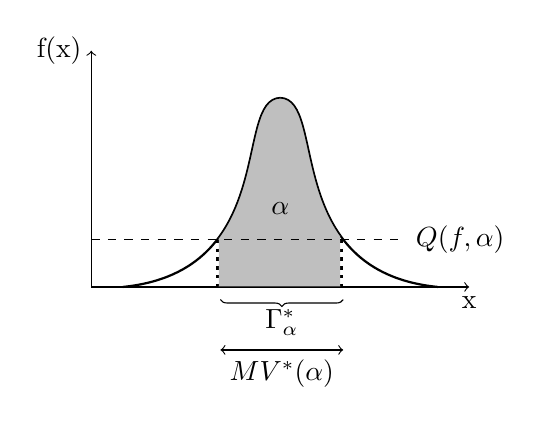
\begin{tikzpicture}[scale=2]

\draw[->](7.8,0)--(10.2,0) node[below]{x};
\draw[->](7.8,0)--(7.8,1.5) node[left]{f(x)}; 
\draw [thick] (8,0) ..controls +(1,0.1) and +(-0.3,-0.01).. (9,1.2);
\draw [thick] (9,1.2) ..controls +(0.3,-0.01) and +(-1,0.1).. (10,0);

\draw[dotted,very thick](8.60,0.3)--(8.60,0) node[right]{};
\draw[dotted,very thick](9.39,0.3)--(9.39,0) node[right]{};

%\draw (8,0.3)--(10,0.3)--(10,1.5)--(8,1.5)--(8,0.3); dessine 4 segments correspondant au 4 points

%hachurage :
\begin{scope} 
\clip (8.61,0)--(9.38,0)--(9.38,1.5)--(8.61,1.5)--(8.61,0) ; %tout ce qui est dans begin{scope} se limitera au rectangle

\path[draw,fill=lightgray] (8,0) ..controls +(1,0.1) and +(-0.3,-0.01).. (9,1.2)--
(9,1.2) ..controls +(0.3,-0.01) and +(-1,0.1).. (10,0)--
(8,0)--(10,0) --cycle;
\end{scope}

\draw[dashed](7.8,0.3)--(9.8,0.3) node[right]{$Q(f,\alpha)$};

%accolade :
\draw[decorate,decoration={brace}]
(9.4,-0.08)--(8.62,-0.08) node[below,pos=0.5] {$\Gamma_\alpha^*$};

\draw[<->]
(9.4,-0.4)--(8.62,-0.4) node[below,pos=0.5] {$MV^*(\alpha)$};



\draw (9,0.5) node[thick]{ $\alpha$} ;
%\draw (8.8,-0.8) node[thick]{Figure 1: MV curve} ;
\end{tikzpicture}
\caption{Masse-Volume au niveau $\alpha$}
\label{resume_fr:MVcurve}
\end{figure}

Pour ce faire, il faut d'abord estimer une collection d'ensembles de volume minimal relatifs aux masses cibles $ 0 <\alpha_1 <\ldots <\alpha_K <1 $ formant une subdivision de $ (0,1) $ sur la base des données d'entrainement afin de définir $s=\sum_k \mathds{1}_{\{x\in \hat \Gamma_{\alpha_k}^*\}}$. L'analyse se fait sous des hypothèses adéquates (relatives à $ \mathcal {G} $, au périmètre de $ \Gamma ^ * _ {\alpha_k} $ et au pas de la subdivision en particulier) et pour un choix approprié de $ K = K_n $.
Cependant, par construction, les vitesse d'apprentissage sont plutôt lentes (de l'ordre $ n ^ {- 1/4} $) et ne peuvent pas être établies lorsque le support n'est pas borné.

Les quatre principaux inconvénients de ce critère de courbe masse-volume sont les suivants.

\begin{itemize}
\item[\textbf{1)}] Lorsqu'il est utilisé comme critère de performance, la mesure de Lebesgue d'ensembles pouvant être très complexes doit être calculée.
\item[\textbf{2)}] Lorsqu'il est utilisé comme critère de performance, il n'existe pas de méthode directe pour comparer les courbes MV puisque l'aire sous la courbe est potentiellement infinie.
\item[\textbf{3)}] Lorsqu'il est utilisé comme critère d'apprentissage, il produit des ensembles de niveau qui ne sont pas nécessairement imbriqués, puis des fonctions de score imprécises.
\item[\textbf{4)}] Lorsqu'il est utilisé comme un critère d'apprentissage, les taux d'apprentissage sont plutôt lents (de l'ordre $ n ^ {- 1/4} $), et ne peuvent pas être établis dans le cas d'un support non borné.
\end{itemize}




Dans la section suivante, et comme contribution de cette thèse, un autre critère fonctionnel est proposé, obtenu en échangeant objectif et contrainte dans \eqref{resume_fr:eq:MV}. Les inconvénients du critère de la courbe masse-volume sont résolus à l'exception du premier, et l'on montre que l'optimisation d'une version discrète empirique de cette mesure de performance donne des fonctions de score avec des taux de convergence de l'ordre $ \mathcal {O} _ {\mathbb {P}} (1 / \sqrt {n}) $. En outre, les résultats peuvent être étendus à la situation où le support de la distribution $ F $ n'est pas compact. De plus, lorsqu'on relaxe l'hypothèse faite dans l'analyse de la courbe masse-volume que tous les ensembles de niveau de $f$ sont inclus dans notre classe de minimisation $ \mathcal {A} $, un contrôle du biais du modèle est établi. Enfin, nous déduisons des propriétés théoriques (non statistiques) vérifiées par ce critère, ce qui corrobore sa qualité de métrique sur les ensembles de niveau contenus dans les fonctions de score.


\subsection{Le critère d'excès de masse}
\label{resume_fr:em-curve}
%The contribution summarized here has been published in~\cite{AISTAT15}.
Nous proposons un autre critère de performance qui s'appuie sur la notion de \textit {d'excès de masse} et d'\textit{ensemble de contours de densité}, comme introduits dans la contribution \cite{Polonik95}. L'idée principale est de considérer une formulation lagrangienne d'un problème de minimisation sous contrainte, obtenu en échangeant la contrainte et l'objectif dans \eqref{resume_fr:eq:MV}: pour $ t> 0 $,

\begin{equation}
\label{resume_fr:solomeg}
\max_{\Omega~ \text{borelien}}  \left\{ \mathbb{P}(\mb X \in \Omega) - t \leb(\Omega) \right\}.
\end{equation}
On désigne par $ \Omega ^ * _ t $ une solution de ce problème. Cette formulation offre certains avantages à la fois computationnels et théoriques: en laissant (une version discrétisée) du multiplicateur lagrangien $ t $ augmenter de $ 0 $ à l'infini, on peut facilement obtenir des solutions à la contrepartie empirique de \eqref{resume_fr:solomeg} formant une suite \textit {imbriquée} d'ensembles, évitant ainsi une dégradation du taux de convergence -- due à la transformation des solutions empiriques pour forcer la monotonie.

%
%\subsubsection{Theoretical study}
La \textbf{courbe d'excès de masse optimale} d'une distribution de probabilité  $F$ est définie comme le graphe de la fonction
$$t>0~~\mapsto~~ EM^*(t):=\max_{\Omega\text{ borelian} } \{ {\mathbb{P}} (\mb X\in \Omega)-t\leb(\Omega) \}.$$ 
Avec les notations précédentes, nous avons: $EM^*(t)=\mathbb{P}(\mb X \in \Omega_t^*)-t \leb(\Omega_t^*)$ pour tout $t>0$.
Remarquons que $EM^*(t) = 0$ pour tout $t>\|f\|_\infty:=\sup_{x\in \rset^d}\vert f(x)\vert$. 
%
  La \textbf{courbe d'excès de masse} de $s\in\mathcal{S}$ par rapport à la distribution de probabilité $F$ d'une variable aléatoire $\mb X$ est le graphe de la fonction
\begin{equation}
\label{resume_fr:EM}
EM_s : t \in [0, \infty[ \mapsto \sup_{A \in \{(\Omega_{s,l})_{l>0}\}}\{ {\mathbb{P}}(\mb X \in A) - t \leb(A)\},
\end{equation}
où $\Omega_{s,t}=\{ x \in \rset^d, s(x) \ge t \}$ pour tout $t>0$.

On peut également écrire $ EM_s $ en termes de $ \lambda_s $ et $ \alpha_s $ définis en \eqref{resume_fr:eq:alpha_beta}, $EM_s(t)= \sup_{u>0}~ \alpha_s(u) -t \lambda_s(u) $. Enfin, sous l'hypothèse $ \mathbf {A_1} $, nous avons $ EM_s (t) = 0 $ pour tout $t> \|f\|_\infty$.

%
\begin{center}
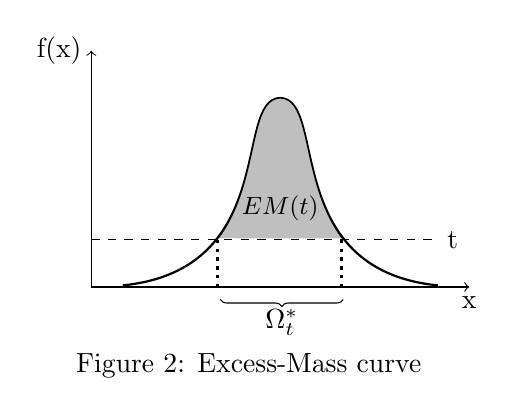
\begin{tikzpicture}[scale=2]
\draw[->](7.8,0)--(10.2,0) node[below]{x};
\draw[->](7.8,0)--(7.8,1.5) node[left]{f(x)}; 
\draw [thick] (8,0.01) ..controls +(1,0.1) and +(-0.3,-0.01).. (9,1.2);
\draw [thick] (9,1.2) ..controls +(0.3,-0.01) and +(-1,0.1).. (10,0.01);
\draw[dashed](7.8,0.3)--(10,0.3) node[right]{t};
\draw[dotted,very thick](8.60,0.3)--(8.60,0) node[right]{};
\draw[dotted,very thick](9.39,0.3)--(9.39,0) node[right]{};
%
%\draw (8,0.3)--(10,0.3)--(10,1.5)--(8,1.5)--(8,0.3); dessine 4 segments correspondant au 4 points
%
%hachurage :
\begin{scope} 
\clip (8,0.31)--(10,0.308)--(10,1.5)--(8,1.5)--(8,0.308) ; %tout ce qui est dans begin{scope} se limitera au rectangle (8,0.3)--(10,0.3)--(10,1.5)--(8,1.5)--(8,0.3)
\path[draw,fill=lightgray] (8,0) ..controls +(1,0.1) and +(-0.3,-0.01).. (9,1.2)--
(9,1.2) ..controls +(0.3,-0.01) and +(-1,0.1).. (10,0)--
(8,0.3)--(10,0.3) --cycle;
\end{scope}

%accolade :
\draw[decorate,decoration={brace}]
(9.4,-0.08)--(8.62,-0.08) node[below,pos=0.5] {$\Omega_t^*$};

\draw (9,0.5) node[]{\small $EM(t)$} ;
\draw (8.8,-0.5) node[thick]{Figure 2: Excess-Mass curve} ;
\end{tikzpicture}
\label{resume_fr:EMcurve}
\end{center}
%
\noindent
Maximiser $ EM_s $ peut être vue comme trouver une collection de sous-ensembles $ (\Omega ^ * _ t) _ {t> 0} $ avec une masse maximale lorsqu'ils sont pénalisés par leur volume de façon linéaire. Une fonction de score optimale est alors n'importe quel $ s \in \S $ admettant $ \Omega^*_t $ 's comme ensembles de niveau, par exemple une fonction de score de la forme
\begin{align*}
%\label{score_cont}
s(x)=\int_{t=0}^{+\infty} \mathds{1}_{x\in \Omega^*_t}a(t)dt,\end{align*}
avec $a(t)>0$ (notons que $s(x)=f(x)$ pour $a \equiv 1$).
%
La fonction $EM_s$ est décroissante sur $(0,+\infty)$, à valeurs dans $[0,1]$ et satisfait, $EM_s(t) \le EM^*(t)$ pour tout $t\geq 0$. 
De plus, pour $t \ge 0$ et pour n'importe quel $\epsilon > 0$, nous avons 
\begin{align*}
%\label{i}
\inf_{u>0} \epsilon \leb (\{ s >u\}\Delta_\epsilon \{f>t\}) &~\le~ EM^*(t)-EM_s(t) \\ &~~~~~~~~~~~~~~~~~~~\le~ \|f\|_\infty \inf_{u>0} \leb (\{ s >u\}\Delta\{f>t\})
\end{align*}
avec $\{ s >u\}\Delta_\epsilon \{f>t\} ~:=~~ \{f>t+\epsilon\} \setminus \{ s >u\} ~~~\bigsqcup~~~ \{ s >u\} \setminus \{f>t-\epsilon\}$. Ainsi la quantité $EM^*(t)-EM_s(t)$ mesure avec quelle qualité les ensembles de niveau de $s$ peuvent-il approchés ceux de la densité sous-jacente.
Sous des hypothèse raisonnables, (voir \cite{AISTAT15}, Prop.1), nous avons aussi pour $\epsilon >0$, 
\begin{align*}
%\label{ii}
\sup_{t\in[\epsilon ,\|f\|_\infty]}|EM^*(t)-EM_s(t)| ~~\le~~  C \inf_{T  \in \mathcal{T}} \|f-T\circ s\|_\infty
\end{align*}

où l'infimum est pris sur l'ensemble $ \mathcal {T} $ de toutes les transformations croissantes mesurables $T: \mathbb {R} _ + \rightarrow \mathbb {R} _ + $.
Les inégalités précédentes révèlent que $ \| EM ^ * - EM_s \| _ \infty $ peut être interprété comme une pseudo distance, soit entre les ensembles de niveau de $ s $ et ceux de la densité sous-jacente $ f $, soit entre les pré-ordres induits par $ s $ et $ f $.

Le concept de la courbe EM fournit un moyen simple de comparer les fonctions de score, mais l'optimisation d'un tel critère fonctionnel est loin d'être simple. Comme proposé dans \cite {CLEM13} pour le critère MV, l'optimisation est faite sur une certaine classe de fonctions de score, que nous espérons assez riche pour fournir une bonne approximation (biais de modèle petit) tout en étant assez simple pour contrôler le taux de convergence. Nous considérons ici les fonctions de score de la forme

\begin{align*}
%\label{score}
s_N(x):= \sum_{k=1}^N a_k \mathds{1}_{x \in \hat{\Omega}_{t_k} }~, ~~~\text{avec ~~~} \hat{\Omega}_{t_k}  \in \mathcal{G}
\end{align*}
où $\mathcal{G}$ est une class VC de sous-ensembles de $\rset^d$.
Nous choisissons de manière arbitraire $a_k:= (t_k-t_{k+1})$ de telle sorte que les $\hat{\Omega}_{t_k}$ correspondent exactement aux ensembles de niveau $t_k$, $\{s \ge t_k\}$. Ensuite, la maximisation du critère fonctionnel d'excès de masse s'effectue en résolvant de manière séquentielle, pour $k=1,\ldots,N$,
\begin{align*}
\hat \Omega_{t_k} \in \argmax_{\Omega \in \mathcal{G}} \frac{1}{n}\sum_{i=1}^n\mathds{1}_{X_i \in \Omega}~-~t_k \leb(\Omega).
\end{align*}

Les solution $ \hat \Omega_ {t_k} $ de ces problèmes d'optimisation peuvent toujours être choisies de manière à être imbriquées (contrairement au problème d'optimisation analogue pour le critère masse-volume). En d'autres termes, une contrainte d'inclusion peut être incorporée dans le problème d'optimisation précédent, sans affecter la qualité de la solution obtenue. Dans le cadre du critère masse-volume, des hypothèses sont faites stipulant que le support de la distribution doit être compact et que la classe VC $ \mathcal {G} $ doit contenir les ensembles de niveau de la densité $f$. Ici, nous relaxons ces hypothèses, la première en choisissant des niveaux adaptatifs $ t_k $, et la seconde en dérivant une étude de biais. %Ceci est détaillé chapitre~\ref{aistat:chap}.



\section{Précision sur les régions extrêmes}
\label{resume_fr:extreme}
\subsection{Analyse du point de vue de la théorie des valeurs extrêmes par l'estimation de la STDF}
\label{resume_fr:stdf}
Cette section est basée sur l'article \cite{COLT15}.

Rappelons que les fonctions de score sont construites en approchant les ensembles de niveau de densité / ensembles de volume minimal de la densité "normale" sous-jacente. Comme nous l'avons mentionné précédemment, dans le cadre de la détection d'anomalie, nous souhaitons être précis sur des ensembles de niveau correspondant à des quantiles élevés, à savoir avec un niveau $ t $ près de $ 0 $ -- ou de manière équivalente, être précis sur des ensembles de volume minimal avec une contrainte de masse $ \alpha $ proche de $ 1 $.

%
Dans le cas univarié, supposons que nous voulons considérer le quantile d'ordre $(1-p)$ de la distribution $ F $ d'une variable aléatoire $ X $, pour une probabilité donnée de dépassement $ p $, c'est-à-dire
 $x_p = \inf\{x \in \mathbb{R},~ \mathbb{P}(X > x) \le p\}$. 
Pour les valeurs modérées de $ p $, une contrepartie empirique naturelle est
 $x_{p,n} = \inf\{x \in \mathbb{R},~ 1/n \sum_{i=1}^n \mathds{1}_{X_i > x}\le p\}$.
Cependant, si $ p $ est très petit, l'échantillon fini $ X_1, \ldots, X_n $ ne contient pas suffisamment d'informations et $ x_ {p, n} $ devient inutile.
%
Ce problème devient dans le cas multivarié celui d'estimer des ensembles de niveau de densité avec un niveau très faible ou de manière equivalente celui d'estimer les fonctions de score associées à ces ensembles de niveau.
%
La théorie des valeurs extrêmes traite spécialement de ces problèmes, aussi bien dans le cadre unidimensionnel que multidimensionnel.
%


\paragraph{Préliminaires.}
La théorie des valeurs extrêmes (nommée dans la suite \textsc {TVE}) développe des modèles pour apprendre l'insolite plutôt que l'habituel. Ces modèles sont largement utilisés dans les domaines de la gestion des risques comme celui de la finance, de l'assurance, des télécommunications ou des sciences de l'environnement. Une application majeure de la \textsc{TVE} est de fournir une évaluation raisonnable de la probabilité d'occurrence d'événements rares.

Pour illustrer ce point, supposons que nous voulons gérer le risque d'un portefeuille contenant $ d $ actifs différents, $ \mb X = (X_1, \ldots, X_d) $. Un but assez général est alors d'évaluer la probabilité d'événements du type
 $\{X_1 \ge x_1 \text{ or }  \dotsc \text{ or } X_d\ge x_d \}$, 
pour des seuils multivariés grands $\mb x=(x_1,\ldots,x_d)$. Dans des conditions pas trop strictes sur la régularité de la distribution $ \mb X $, la \textsc {TVE} montre que pour des seuils suffisamment importants,
\[
\P\{X_1 \ge x_1 \text{ or }  \dotsc \text{ or }
X_d\ge x_d \} \simeq 
l(p_1,\ldots,p_d), 
\] 
où $ l $ est la STDF (\emph{stable tail dependence function}) et où les $ p_j $  sont les probabilités de dépassement marginal, $ p_j = \P (X_j \ge x_j) $. La fonction $ l $ caractérise la \emph {dépendance} entre les extrêmes. La distribution \emph {jointe} (sur des seuils importants) peut donc être récupérée à partir de la connaissance des distributions marginales avec la \textsc {stdf} $ l $. Dans la pratique, $ l $ peut être estimée à partir de données "modérément extrêmes", typiquement les $ k $ `plus grandes 'parmi un échantillon de taille $ n $, avec $ k \ll n $.

L'estimation des $ p_j $ peut s'effectuer suivant un chemin bien pavé: dans le cas univarié, la \textsc {TVE} consiste essentiellement à modéliser la distribution des maxima (\emph {resp.} la queue de distribution) par un élément des familles paramétriques de Gumbel, Fréchet ou Weibull (\emph {resp.} par une distribution de Pareto généralisée).

Par contre, dans le cas multivarié, il n'y a pas de paramétrisation fini-dimensionnelle de la structure de dépendance.
Cette dernière étant caractérisée par la \textsc {stdf}, l'estimation de cette fonctionnelle est l'un des principaux problèmes de la \textsc {TVE} multivariée. Les propriétés asymptotiques de la contrepartie empirique de la \textsc {stdf} ont été largement étudiées, voir \cite {Huangphd, Drees98, Embrechts2000, dHF06} pour le cas bivarié et \cite {Qi97, Einmahl2012} pour le cas général multivarié sous des hypothèses de régularité.

Cependant, aucune borne n'existe sur l'estimation non-asymptotique. La contribution résumée dans la section suivante et publiée dans \cite{COLT15} dérive de telles bornes non asymptotiques. Nos résultats ne nécessitent aucune hypothèse autre que l'existence de la \textsc {stdf}.


\paragraph{Apprentissage de la structure de dépendance des événements rares.}
Les inégalités de VC classiques visent à borner la déviation des quantités empiriques par rapport aux quantités théoriques sur des classes d'ensemble relativement simples, appelées classes VC. Assez souvent, ces classes recouvrent tout le support de la distribution sous-jacente. Cependant, lorsqu'il s'agit d'événements rares, il est intéressant d'avoir de telles bornes sur une classe d'ensembles qui ne couvre qu'une région de faible probabilité et contient donc (très) peu d'observations. Cela donne des bornes plus fines, puisque seules les différences entre de très petites quantités sont impliquées dans l'analyse. Le point de départ est l'inégalité VC énoncée ci-dessous. %et prouvée dans le chapitre~\ref{colt}.

\begin{theoreme}
\label{resume_fr:thm-princ} 
Soit $\mathbf{X}_1,\ldots,\mathbf{X}_n$ des réalisations \iid~d'une variable aléatoire $\mathbf{X}$, $\mathcal{A}$  une classe VC de VC-dimension $V_{\mathcal{A}}$. 

Considerons la classe $\mathbb{A} = \cup_{A \in \mathcal{A}} A$, et posons $p = \mathbb{P}(\mathbf{X} \in \mathbb{A})$. 
Alors il existe une constante absolue $ C $ de sorte que pour tout $ 0 <\delta <1 $, avec probabilité au moins $ 1- \delta $,
\begin{align*}
\sup_{A \in \mathcal{A}} \left| \mathbb{P} \big[\mathbf{X} \in A\big] - \frac{1}{n} \sum_{i=1}^n \mathds{1}_{\mathbf{X}_i \in A}  \right| ~~\le~~ C \bigg[ \sqrt{p}\sqrt{\frac{V_{\mathcal{A}}}{n} \log{\frac{1}{\delta}}} + \frac{1}{n} \log{\frac{1}{\delta}} \bigg]~.
\end{align*}
\end{theoreme}

L'idée principale est la suivante. L'estimateur empirique de la {\sc stdf} est basé sur la mesure empirique des régions "extrêmes", qui sont touchées seulement avec une faible probabilité. Il suffit donc de borner les déviations maximales sur ces régions à faible probabilité.
La clé consiste à choisir une classe VC adaptative, qui ne couvre que ces régions là, et à dériver des inégalités de type VC qui intègrent $p$, la probabilité de toucher la classe. La borne obtenue sur l'erreur non asymptotique est alors:

\begin{theoreme}
\label{resume_fr:thm:l}
Soit $T$ un nombre positif tel que $T \ge \frac{7}{2}(\frac{\log d}{k} + 1)$, $\delta$ tel que $\delta \ge e^{-k}$ et soit $k=k(n)$ une suite d'entiers strictement positifs telle que $k \to \infty$ et $k=o(n)$ quand $n \to \infty$. 
Alors il existe une constante absolue $ C $ telle que pour chaque $ n> 0 $, avec probabilité au moins $ 1- \delta $:
\begin{align*}
\sup_{0 \le \mathbf{x} \le T} \left| l_n(\mathbf{x}) - l(\mathbf{x}) \right| ~\le~ Cd\sqrt{\frac{T}{k}\log\frac{d+3}{\delta}} ~+~
\text{bias}(k, n, T),
\end{align*}
où $ l $ est la \stdf~et $ l_n $ sa version empirique standard. Le second terme dans la borne est un biais issu de la nature asymptotique de $ l $.
\end{theoreme}


Dans cette section, nous avons introduit et étudié, dans un cadre non-paramétrique, une fonctionnelle particulière caractérisant la structure de dépendance des extrêmes.
%
Une autre caractérisation pratique (non paramétrique) de cette dépendance dans le cadre de la TVE multivariée est la \textit{mesure angulaire} qui fournit des informations directes sur les "directions" probables des extrêmes, c'est-à-dire la contribution relative de chaque coordonnée dans les "grandes" observations.

Dans de nombreuses applications, il est plus commode de travailler avec la mesure angulaire elle-même. Cette dernière donne des informations plus directes sur la structure de dépendance et est capable de refléter des propriétés structurelles (par exemple la sparsité/parcimonie comme détaillé ci-dessous) qui n'apparaîtraient pas dans les copules ou dans la STDF, ces derniers étant des versions intégrées de la mesure angulaire.
Cependant, la modélisation non paramétrique de la mesure angulaire est confrontée à des difficultés majeures, dues à sa structure potentiellement complexe, en particulier dans un cadre de grande dimension.
D'autre part, d'un point de vue théorique, l'estimation non paramétrique de la mesure angulaire n'a été étudiée que dans le cas bidimensionnel et dans un cadre asymptotique \cite{Einmahl2001, Einmahl2009}. La section ci-dessous résume une nouvelle méthodologie visant à représenter parcimonieusement la structure de dépendance des extrêmes.


\subsection{Représentation parcimonieuse des extrêmes multivariés}
\label{resume_fr:sec:JMVA}
Cette section résume les travaux publiés \cite{AISTAT16}, ainsi que sa version longue \cite{ARXIV16} en cours de révision.

La TVE a été intensivement utilisée en détection d'anomalies dans le cas unidimensionnelle, voir par exemple \cite{Roberts99, Roberts2000, Clifton2011, Clifton2008, Lee2008}. Dans le cas multivariée, cependant, il n'existe -- à notre connaissance -- aucune méthode de détection d'anomalies reposant sur la TVE \textit {multivariée}. Jusqu'à présent, le cas multidimensionnel n'a été abordé que par l'usage de statistiques basées sur la TVE univariée. La raison majeure est la difficulté du passage à l'échelle des modèles multivariés avec la dimension. Dans le présent travail, nous comblons l'écart entre la détection d'anomalies et la TVE multivariée en proposant une méthode qui est capable d'apprendre un "profil normal" parcimonieux des extrêmes multivariés et, en tant que tel, peut être mis en œuvre pour améliorer la précision de tout algorithme de détection d'anomalies.\\


\textbf{Context: Extrèmes multivariés en grande dimension.}
%\label{context}
L'estimation paramétrique ou semi-paramétrique de la structure des extrêmes multivariés est relativement bien documentée dans la littérature, voir par exemple
\cite{coles1991modeling,fougeres2009models,cooley2010pairwise,sabourinNaveau2012} 
et leurs références. Cependant, des hypothèses structurelles restrictives doivent être faites, stipulant par exemple que seuls quelques sous-groupes pré-définis de composantes peuvent être extrêmes ensemble. %, ou au contraire, que toutes doivent l'être. 
En outre, leur utilisation pratique est limitée à des problèmes en dimension modérée (par exemple, $ d \le 10 $), sinon des choix de modélisation simplifiés sont nécessaires -- comme dans \cite {stephenson2009high}. Enfin, l'évaluation de l'incertitude concernant les quantités produites par ces modèles est faite sous l'hypothèse que les données d'entraînement sont "asymptotiques", au sens où l'on suppose que, quand elles excèdent un grand seuil fixé, les données sont exactement réparties selon la distribution limite des extrêmes . En d'autres termes, l'erreur de modélisation est ignorée.


L'estimation non-paramétrique de la mesure angulaire n'a été traitée que dans le cas bidimensionnel, dans \cite{Einmahl2001, Einmahl2009}, et dans un cadre asymptotique. Nous allons étendre l'étude non-asymptotique sur l'estimation de la {\sc stdf} (section précédente) à la mesure angulaire des extrêmes, restreinte à une classe bien choisie d'ensembles. L'objectif est d'apprendre une représentation de la mesure angulaire, assez simple pour contrôler la variance en grande dimension et suffisamment précise pour obtenir des informations sur les "directions probables" des extrêmes. Ceci donne une première estimation non paramétrique de la mesure angulaire en dimension quelconque, limitée à une classe de sous-cones, avec une borne non asymptotique sur l'erreur.
Notons que ce procédé peut également être utilisé comme étape de prétraitement, dans un cadre de réduction de  dimension, avant de procéder à une estimation paramétrique ou semi-paramétrique qui pourrait bénéficier des informations de structure émises lors de la première étape. De telles applications dépassent le cadre de cette thèse.

Le cadre que nous développons est non paramétrique et se trouve à l'intersection de l'estimation de support, de l'estimation de densité et de la réduction de dimension: il consiste à apprendre le support d'une distribution (à partir des données d'apprentissage),  qui peut être décomposé en sous-cones, potentiellement de dimension faible et auxquels une certaine masse est assignée.%, définissant des versions empiriques de probabilité sur régions extrêmes.

Ceci produit une fonction de score définie sur les régions extrêmes, qui peut ainsi être exploitée pour détecter les anomalies parmi les extrêmes.
En raison de sa complexité modérée - d'ordre $ dn \log n $ - cet algorithme convient au traitement de problèmes d'apprentissage à grande échelle, et les résultats expérimentaux révèlent une performance significativement accrue sur les régions extrêmes par rapport aux approches de détection d'anomalies standards.


Dans un large éventail de situations, on peut s'attendre à l'apparition de deux phénomènes:

\textbf{1-} Il y a seulement un "petit" nombre de groupes de coordonnées pouvant être extrêmes ensemble, de sorte que seul un "petit" nombre d'hyper-cubes (ceux correspondant à ces sous-ensembles de coordonnées) ont une masse non nulle -- "petite" est relatif au nombre total de groupes, $2^d$.

\textbf{2-} Chacun de ces groupes contient un nombre limité de coordonnées (par rapport à la dimension initiale), de sorte que les hyper-cubes correspondants (de masse non nulle) ont une petite dimension par rapport à $ d $.

Le but principal de ce travail est d'introduire une méthodologie pilotée par les données pour identifier ces groupes, afin de réduire la
dimension du problème et ainsi apprendre une représentation parcimonieurse des comportements extrêmes.

Dans le cas où l'hypothèse \textbf{2-} n'est pas vérifiée, une telle représentation peut tout de même être apprise, mais perd la propriété que les hyper-cubes la supportant sont de faible dimension.

Un problème majeur est que les données réelles ne se concentrent généralement pas sur les sous-espaces de mesure Lebesgue nulle. Ceci peut être résolu en mettant à zéro n'importe quelle coordonnée inférieure à un seuil $ \epsilon> 0 $, de sorte que "l'angle" correspondant soit affecté à une face de dimension inférieure.

Plus formellement, les figures \ref{resume_fr:fig:3Dcones} et \ref{resume_fr:2Dcones} représentent l'espace initial des données transformé, résultant de la standardisation classique des marginales. Après cette transformation non linéaire, la représentation des données extrêmes est pour sa part linéaire et apprise en estimant la masse portée par les sous-cônes
%
\begin{align*}
 \mathcal{C}_\alpha = \{\mb v \ge 0,~\|\mb v\|_\infty \ge 1,~ v_j > 0 ~\text{ for } j \in \alpha,~ v_j = 0 ~\text{ for } j \notin \alpha \},
\end{align*}
ou plus précisément, la masse de la mesure angulaire $\Phi$ sur les sous-sphères correspondantes
\begin{align*}
\Omega_{\alpha}  = \{\mb x \in S_{\infty}^{d-1} :  x_i > 0 \text{ for } i\in\alpha~,~  x_i = 0 \text{ for } i\notin \alpha   \} 
 = S_{\infty}^{d-1}\cap {\mathcal{C}}_\alpha,
\end{align*}
représentées Figure~\ref{resume_fr:fig:3Dcones}.

\begin{minipage}{0.5\linewidth}
\centering
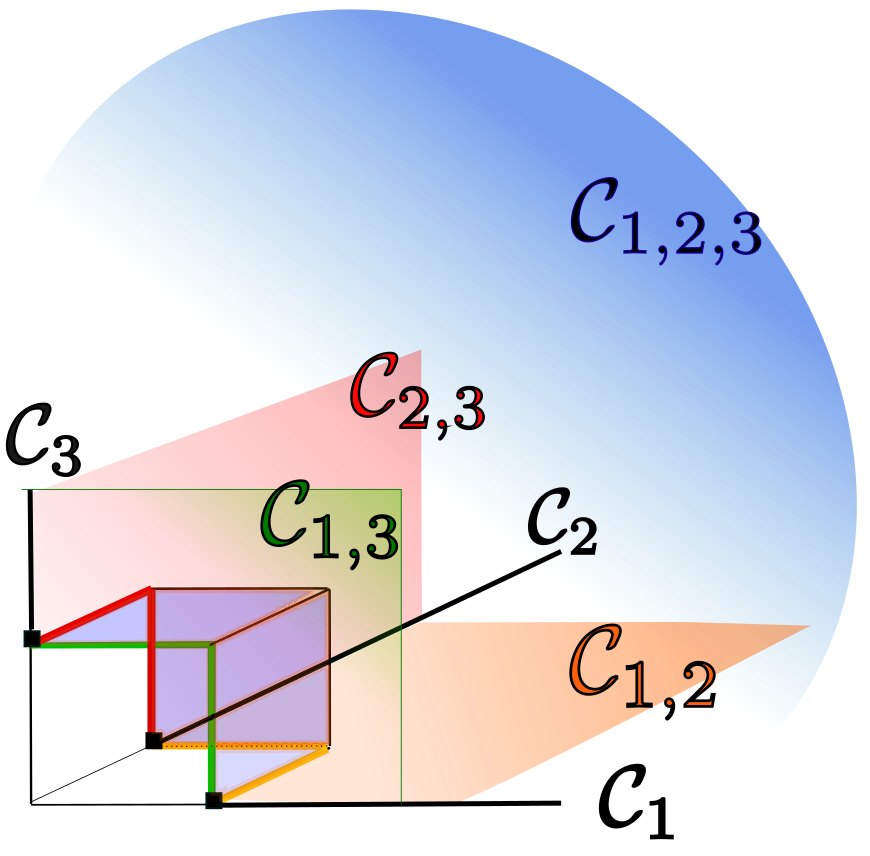
\includegraphics[scale=0.2]{fig_source/cone}
\captionof{figure}{Truncated cones in 3D}
\label{resume_fr:fig:3Dcones}
\end{minipage}\hfill
\begin{minipage}{0.5\linewidth}
\centering
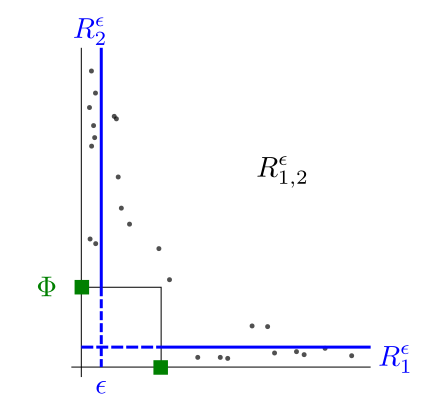
\includegraphics[width=0.64\linewidth]{fig_source/representation2D}
\captionof{figure}{Truncated $\epsilon$-cones in 2D}
\label{resume_fr:2Dcones}
\end{minipage}

~\\
Cette estimation est faite en utilisant les sous-cones $\epsilon$-épaissis $\cone_\alpha^\epsilon$, correspondant aux sous-sphères $\epsilon$-épaissies $\Omega_\alpha^\epsilon$, comme le montre la Figure~\ref{resume_fr:2Dcones} dans le cas de la dimension deux.
Nous obtenons ainsi un estimateur $\widehat{\mathcal{M}}$ de la représentation
$$\mathcal{M} = \{ \Phi(\Omega_{\alpha}):\; \emptyset \neq \alpha\subset\{1,\; \ldots,\; d \}\}.$$
Théoriquement, retrouver le vecteur inconnu $\mathcal{M}$ de dimension $(2^{d}-1)$ revient à peu près à approximer le support de $\Phi$ en utilisant la partition
$\{\Omega_\alpha, \alpha\subset\{1,\ldots,d\}, \alpha\neq \emptyset\}$, c'est-à-dire, déterminer quels sont les $\Omega_\alpha$ qui ont
une masse non nulle -- et évaluer cette masse $\Phi(\Omega_\alpha)$. %, ou de manière équivalente, déterminer quels sont les $\Phi_\alpha$ non nuls. 
Cette estimation de support est potentiellement parcimonieuse -- si seul un petit nombre d'$\Omega_\alpha$ ont une masse non nulle, \ie~Phénomène~\textbf{1-} -- et
potentiellement de faible dimension -- si les dimensions des sous-sphère $\Omega_\alpha$ ayant une masse non nulle sont faibles comparées à $d$, \ie~Phénomène~\textbf{2-}.

% Second, investigate how the angular measure $\Phi$ spreads its mass on the
% $\Omega_{\alpha}$'s, the theorical quantity $\Phi(\Omega_{\alpha})$ indicating to which extent extreme observations may occur in the `direction' $\alpha$ for $\emptyset \neq \alpha \subset \{1,\; \ldots,\; d \}$. 

% These two goals are achieved using empirical versions of
% the angular measure, evaluated on the $\epsilon$-thickened sub-spheres $\Omega_\alpha^\epsilon$.

\textbf{Détection d'anomalies.}
L'algorithme que nous proposons, DAMEX (Detecting Anomalies with Extremes), apprend une représentation $\widehat{\mathcal{M}}$ (éventuellement parcimonieuse et de faible dimension) de la mesure angulaire, à partir de laquelle une fonction de score peut être définie dans le contexte de la détection des anomalies.
L'hypothèse sous-jacente est qu'une observation est potentiellement anormale si sa "direction" (après une normalisation de chaque marginal) est particulière par rapport aux autres observations extrêmes. En d'autres termes, si elle n'appartient pas à la représentation (parcimonieuse) $\widehat {\mathcal {M}} $. %Plus de détails sur la façon dont la fonction de score est définie à partir de cette représentation peuvent être trouvés dans le chapitre correspondant.
Selon les expériences obtenus dans ce chapitre, DAMEX améliore significativement les performances (en terme de précision et de courbes ROC) dans les régions extrêmes, ce qui induit des courbes ROC plus verticales près de l'origine.

\textbf{Garanties théoriques.}
A partir des travaux sur l'estimation de la \stdf~résumés dans la sous-section précédente~\ref{resume_fr:stdf}, en particulier à partir du Théorème~\ref{resume_fr:thm-princ} et des idées utilisées pour prouver le Théorème~\ref{resume_fr:thm:l}, nous sommes en mesure de prouver quelques garanties théoriques relative à cette approche.
%
Sous des hypothèses non-restrictives standards en TVE (existence de la mesure angulaire et fonctions de répartition des marges continues), on obtient une borne non asymptotique de la forme
\begin{align*}
\sup_{\emptyset \neq \alpha \subset \{1,\; \ldots,\; d \}}~ |\widehat{\mathcal{M}}(\alpha)- \mathcal{M}(\alpha)|
~\le~  C d \left( \sqrt{ \frac{1}{\epsilon k}\log\frac{d}{\delta}} + M d\epsilon \right) + \text{bias}(\epsilon, k, n),
\end{align*}
avec probabilité plus grande que $1-\delta$, où $k = k(n) \to \infty$ avec $k(n) = o(n)$ pouvant être interprété comme le nombre de données considérées extrêmes.
Le terme de biais tend vers zéro quand $n \to \infty$, pour tout $\epsilon$ fixé.


\section{Approches heuristiques}
\label{resume_fr:sec:heuristic}

Les deux contributions de cette section sont de nature heuristique et ne sont pas encore étayées par des résultats théoriques statistiquement solides. Bien que ces travaux en cours n'aient pas encore été publiés et seront certainement achevés dans un proche avenir, nous pensons qu'ils ont leur place dans ce manuscrit, étant donné les nombreuses expériences numériques convaincantes qui ont été menées et la justification des approches promues.
%
Ces deux contributions abordent deux défis majeurs en détection d'anomalies:

\begin{itemize}
\item Comment évaluer la détection d'anomalies non supervisée en pratique?
\item Comment créer des forêts aléatoires efficaces sur une seule classe de données?
\end{itemize}

Le premier point a été partiellement traité dans la section ~\ref{resume_fr:scoring} avec les courbes MV et EM.
Cependant, ces deux critères ont été initialement introduits pour construire des fonctions de scores \emph{via} minimisation du risque empirique (ERM), et aucune étude n'a été faite sur leur utilisation pour évaluer les fonctions de scores comme le font les critères ROC ou PR dans le cas où des données labélisées sont disponibles.
En outre, leur utilisation pour mesurer la qualité d'une fonction de score $s_n$ implique le calcul de la mesure de Lebesgue $\leb(s_n\ge u) $, ce qui est très difficile quand la dimension est grande.

Les deux approches proposées sont heuristiques, et aucune garantie théorique de consistence ou de taux de convergence n'est dérivée. Cependant, de nombreuses expériences montrent la pertinence de ces approches.

\subsection{Évaluer un algorithme de détection d'anomalies}
\label{resume_fr:evaluation}
Cette partie est basée sur un article de workshop \citep{ICMLworkshop16} et sur un article à soumettre \citep{NIPS16evaluation}.


Lorsque suffisamment de données labélisées sont disponibles, les critères classiques basés sur les courbes ROC \citep{Provost1997, Provost1998, Fawcett2006} ou PR \citep{Davis2006, Clemencon2009} peuvent être utilisés pour comparer les performances d'algorithmes de détection d'anomalies non supervisés. Cependant, dans de nombreuses situations, pas ou peu de données sont étiquetées. C'est dans ce cas qu'un critère alternatif pouvant être calculé sur des données non-étiquetées trouve toute son utilité.

Alors que les courbes d'excès de masse et masse-volume ont été initialement introduites pour construire des fonctions de score \emph{via} minimisation du risque empirique (ERM), la courbe MV a été utilisée récemment pour la calibration du SVM à une classe \citep{Thomas2015}.
Lorsque ce critère est utilisé pour attester la qualité d'une fonction de score, les volumes induits deviennent inconnus et doivent être estimés, ce qui est difficile en grande dimension si aucune connaissance préalable sur la forme de ces ensembles de niveau n'est disponible.
%
De plus, l'efficacité des courbes EM ou MV comme critères d'évaluation n'a pas encore été étudiée.
%
Dans cette section et en tant que contribution de cette thèse, on montre que des scores numériques associées aux critères EM et MV (qui ne nécessitent pas d'étiquettes) sont aptes à discriminer avec précision les algorithmes suivants leurs performances.
%
Une méthodologie basée sur le sous-échantillonnage et l'agrégation de features est également décrite et testée. Elle étend l'utilisation de ces critères à des ensembles de données de grande dimension et résout les principaux inconvénients inhérents aux courbes EM et MV classiques.

Rappelons que les courbes MV et EM d'une fonction de score $s$ peuvent être écrites comme

\begin{align}
\label{resume_fr:intro:MV-def}
 MV_s(\alpha) &= \inf_{u \ge 0}~~ \leb(s \ge u) ~~\st~~\mathbb{P}(s(\mb X) \ge u) \ge \alpha\\
\label{resume_fr:intro:EM-def}
 EM_s(t) &= \sup_{u \ge 0}~~ \mathbb{P}(s(\mb X) \ge u) ~-~ t \leb(s \ge u)
\end{align}

pour tout $\alpha\in (0,1)$ et $t >0$.
%
Les courbes optimales sont $MV^* = MV_f = MV_{T \circ f}$ et $EM^* = EM_f = EM_{T \circ f}$ pour toute transformation croissante $T: \text{Im(f)} \to \mathbb{R}$.
%
Comme il n'existe pas de manière triviale pour comparer deux courbes, considérons la norme $\|.\|_{L^1(I)}$ avec $I\subset \rset$ un interval. Comme $MV^*=MV_f$ est en dessous de $MV_s$ en tout point, $\argmin_s \| MV_s - MV^* \|_{L^1(I)} = \argmin \| MV_s \|_{L^1(I)} $. Nous définissons donc
$\crit^{MV}(s) = \| MV_s \|_{L^1(I^{MV})},$ ce qui revient à considérer $\| MV_s - MV^* \|_{L^1(I^{MV})}$. % comme mentionné en introduction. 
Etant donné que nous sommes intéressés par les grands ensembles de niveau, un interval naturel serait par exemple $I^{MV} = [0.9, 1]$. Cependant, la courbe MV diverge en $1$ quand le support est infini, ce qui nous amène à consider arbitrairement $I^{MV} = [0.9, 0.999].$
Plus la valeur de $\crit^{MV}(s)$ est petite, meilleure est la fonction de score $s$.
%
De même, nous considérons $\crit^{EM}(s) = \|EM_s\|_{L^1(I^{EM})},$ cette fois avec $I^{EM} = [0,EM^{-1}(0.9)],$ où $EM_s^{-1}(0.9) := \inf\{t\ge 0,~ EM_s(t) \le 0.9\}$, puisque $EM_s(0)$ est fini (égal à $1$). 

% We point out that such small values of $t$ correspond to large level-sets. Also in practice, we have observed that
% $EM_s^{-1}(0.9)$ (as well as $EM_f^{-1}(0.9)$) varies significantly depending on the dataset. Generally, for datasets in large dimension, it can be % $\widehat{EM}_s^{-1}(0.9)$ is
% very small (in the experiments, smallest values are of order $10^{-7}$) as it is of the same order of magnitude as the inverse of the total support volume.

Comme la distribution $F$ des données normales est généralement inconnue, les courbes MV et EM doivent être estimées.
Soit $s\in \mathcal{S}$ and $\mb X_1,\; \ldots,\; \mb X_n$ un échantillon  i.i.d. de distribution $F$. Utilisons la notation $\mathbb{P}_n(s \ge t)=\frac{1}{n}\sum_{i=1}^n\mathds{1}_{s(\mb X_i)\geq t}.$ 
Les courbes empiriques MV et EM de $s$ sont alors simplement définies comme la version empirique de \eqref{resume_fr:intro:MV-def} ou de \eqref{resume_fr:intro:EM-def}, 
\begin{align}
\label{resume_fr:MV-def-emp}
\widehat{MV}_s(\alpha) = \inf_{u \ge 0} \left\{ \leb(s \ge u) ~~\st~ \mathbb{P}_n(s \ge u) \ge \alpha \right\}
\end{align}
\begin{align}
\label{resume_fr:EM-def-emp}
\widehat{EM}_s(t) = \sup_{u \ge 0} \mathbb{P}_n(s \ge u) ~-~ t \leb(s \ge u)
%\lambda_s \circ \alpha_s^{-1}(\alpha),
\end{align}
%
%
Enfin, nous obtenons les critères de performance empiriques relatifs à EM et MV:
\begin{align}
\label{resume_fr:eq:standard_emp_EM}\widehat{\crit}^{EM}(s) &= \| \widehat{EM}_s \|_{L^1(I^{EM})}  &&I^{EM} = [0,\widehat{EM}^{-1}(0.9)],\\
\label{resume_fr:eq:standard_emp_MV}\widehat{\crit}^{MV}(s) &= \| \widehat{MV}_s \|_{L^1(I^{MV})}  &&I^{MV} = [0.9, 0.999].
\end{align}
%
% As the distribution $F$ is generally unknown, excess-mass curves must be estimated. Let $s\in \S$ and $\mb X_1,\; \ldots,\; \mb X_n$ be an i.i.d. sample with common distribution $F$ and set $$\widehat{\alpha}_s(t)=(1/n)\sum_{i=1}^n\mathds{1}_{s(X_i)\geq t}.$$ The empirical $EM$ curve of $s$ is then defined as $$\widehat{EM}_s(t)=\sup_{u>0}\{ \widehat{\alpha}_s(u)-t\lambda_s(u)\}.$$ In practice, just as with the mass-volume criterion (drawback \textbf{1}), it may be difficult to estimate the volume $\lambda_s(u)$ and Monte-Carlo approximation can naturally be used for this purpose.

% Note that in practice, the volume $\leb(s \ge u)$ is estimated using Monte-Carlo approximation, which only applies to small dimensions.
% %
% This is a major drawback for the use of excess-mass or mass-volume criteria in high dimensional framework, if no prior knowledge on the form of these level sets is available. Besides, there has been no work yet dealing with EM or MV curves as evaluation criteria, as they have originally been introduced to build scoring scoring function via ERM.
%

La méthodologie pour faire passer à l'échelle l'utilisation des critères EM et MV (aux données en grande dimension) consiste à sous-échantillonner les données d'entrainement \emph{et} de test, en utilisant un paramètre $d'$ contrôlant le nombre de dimensions choisies au hasard pour le calcul du score (EM ou MV).
Ce tirage se fait sans remplacement -- le remplacement se fait seulement après chaque tirage $ F_1, \ldots, F_ {m} $.

Un score partiel $\widehat \crit_k^{MV}$ (resp. $\widehat \crit_k^{EM}$) est calculé à chaque tirage $F_k$ en utilisant \eqref{resume_fr:eq:standard_emp_EM} (resp. \eqref{resume_fr:eq:standard_emp_MV}). Le critère de performance final est obtenu en moyennant ces critères partiels. Cette méthodologie est décrite par l'algorithme~\ref{resume_fr:algo:EMMV}.
%
\begin{algorithm}[!tbh]
\caption{~~EM/MV en grande dimension: évaluation d'algorithmes de détection d'anomalies sur des donnéees de dimension élevée}
\label{resume_fr:algo:EMMV}
\begin{algorithmic}
  \STATE \textbf{Entrées}: algorithme de détection d'anomalies $\mathcal{A}$, jeu de données $X = (x^j_i)_{1 \le i \le n, 1 \le j \le d }$, taille de sous-échantillonage $d'$, nombre de tirages $m$.
  \FOR{$k=1,\ldots,m$}
    \STATE{sélectionner aléatoirement un sous-groupe $F_k$ de $d'$ coordonnées}
    \STATE{calculer la fonction de score associée $\widehat s_{k} = \mathcal{A}\big((x^j_i)_{1 \le i \le n,~j \in F_k}\big)$}
    \STATE calculer $\widehat{\crit}_k^{EM} = \| \widehat{EM}_{\widehat s_k} \|_{L^1(I^{EM})}$ en utilisant \eqref{resume_fr:eq:standard_emp_EM} ou $\widehat{\crit}_k^{MV} = \| \widehat{MV}_{\widehat s_k} \|_{L^1(I^{MV})}$ en utilisant \eqref{resume_fr:eq:standard_emp_MV}
  \ENDFOR 
  \STATE \textbf{Sortie}: critère de performance sur $\mathcal{A}$: $$\widehat{\crit}^{EM}_{high\_dim} (\mathcal{A})= \frac{1}{m} \sum_{k=1}^m\widehat \crit_k^{EM} \text{~~~~(idem for MV)}$$
\end{algorithmic}
\end{algorithm}

Les critères EM/MV pour dimension faible et pour dimension élevée sont testés à l'aide de trois algorithmes de détection d'anomalies classiques. Une large gamme de jeux de données étiquetés réels est utilisée à titre de comparaison.
Les expériences montrent que lorsqu'un algorithme a de meilleures performances que d'autres sur un certain jeu de données ("meilleures" selon les AUC des courbes ROC et PR), on peut s'attendre à le retrouver sans utiliser d'étiquettes avec une précision de $82\% $ dans le cadre de détection de nouveauté, et avec une précision de $77\%$ dans le cadre non-supervisé.


\subsection{Forêts aléatoires à une classe}
\label{resume_fr:ocrf}
Cette partie est basée sur un travail en voie de soumission \citep{OCRF16}.

%Scoring functions built by optimizing EM or MV criteria usually not perform well. 

Construire des fonctions de score précises en optimisant les critères EM ou MV est très difficile en pratique, de manière analogue à la construction de classifieurs en optimisant la courbe ROC (\cite{Clemencon2010}) dans le cadre supervisé.
%
Il faut davantage de travail pour que ces méthodes soient efficaces dans la pratique, en particulier au niveau du  choix de la classe d'ensembles sur lesquels l'optimisation est effectuée.
En effet, cette classe doit être \emph{assez riche pour fournir une bonne approximation tout en étant assez simple pour contrôler le taux de convergence}. Ce compromis est difficile à réaliser, en particulier en dimension élevée, lorsqu'aucune connaissance préalable sur la forme des ensembles de niveau n'est disponible.

Dans cette section, nous proposons une approche heuristique pour construire des fonctions de score en utilisant des forêts aléatoires (dans la suite abrégées RF pour "random forests") \citep{Breiman2001, Genuer2008, Biau2008, Biau2016}.
Plus formellement, nous adaptons les RFs au cadre de la classification à une classe en introduisant des critères de séparation à une classe.

Les RFs standards sont des estimateurs qui entrainent un certain nombre de classificateurs d'arbre de décision sur différents sous-échantillons aléatoires de l'ensemble de données. Chaque arbre est construit récursivement, selon un critère de séparation/scission basé sur une certaine mesure d'impureté définie sur chaque noeud de l'arbre -- un noeud est en fait une cellule rectangulaire de l'espace des observations. La prédiction est faite en moyennant les prédictions de chaque arbre. Dans le cadre de la classification (à deux classes), les prédictions des arbres sont moyennés à travers un vote majoritaire. Peu de tentatives pour transférer l'idée des RFs à la classification à une classe ont déjà été faites \citep{Desir12, Liu2008, Shi2012}. Aucun algorithme ne prolonge structurellement (sans échantillonnage de seconde classe et sans estimateurs de base alternatifs) les RFs au cadre de la classification à une classe.

Nous introduisons précisément une telle méthodologie. Elle s'appuie sur une adaptation naturelle des critères de scission à deux classes au contexte de classification à une classe, ainsi qu'une adaptation du vote majoritaire. De plus, il s'avère que le modèle à une classe que nous promouvons ici correspond au comportement asymptotique d'une méthode pour générer des outliers qui s'adapte au données (plus précisement qui s'adapte au processus de croissance des arbres, qui lui dépend des données).

\textbf{Modèle à une classe de paramètres ($n$, $\boldsymbol{\alpha}$), M($n$, $\boldsymbol{\alpha}$).}
Considérons un variable aléatoire $ X:\Omega \to \mathbb{R}^d$ par rapport à un espace probabilisé $(\Omega, \mathcal{F}, \mathbb{P})$.
La loi de $X$ est supposée dépendre d'une autre variable $y \in \{0,1\}$, qui vérifie $\mathbb{P}(y=1)=1-\mathbb{P}(y=0)=\alpha$. Nous supposons que conditionellement à $y=0$, $X$ suit une loi $F$, et conditionellement à $y=1$, une loi $G$:
\begin{align*}
 X ~|~ y=0 ~~\sim~~ F, &~~~~~~~~~~  \mathbb{P}(y=0)=1-\alpha, \\
 X ~|~ y=1 ~~\sim~~ G, &~~~~~~~~~~  \mathbb{P}(y=1)=\alpha.
\end{align*}
%
Nous modélisons le cadre à une classe comme suit. Parmi les $n$ observations \iid nous observons seulement celles avec $y = 0$ (le comportement normal), c'est-à-dire $N$ réalisations de $ (X ~ | ~ y = 0)$ où $N$ est lui-même la réalisation d'une variable aléatoire $\mb N$ de loi $\mb N \sim \text{Bin}\big(n, (1-\alpha)\big)$, la distribution binomiale de paramètres $ (n, P)$. Comme les outliers ne sont pas observés, on suppose classiquement que $G$ suit une distribution uniforme sur l'hyper-rectangle $ \mathcal{X} $ contenant toutes les observations, de sorte que $ G $ a une densité constante $g(x) \equiv 1 / \leb(\mathcal{X})$ sur $\mathcal{X}$. Cette hypothèse \emph{sera supprimée} dans l'approche adaptative, où aucune distribution préalable n'est supposée pour les outliers.
%laisser une ligne car fin du model one class

On obtient alors des analogues empiriques à une classe des mesures d'impuretés à deux classes en remplaçant les quantités relatives au comportement normal par leurs versions empiriques. Les quantités relatives à la deuxième classe non observée (comportement anormal) sont exprimées naturellement en utilisant l'hypothèse de distribution uniforme.

De cette façon, notre fonction de différence d'impuretés à une classe correspond à celle à deux classe, où les quantités empiriques de la seconde classe ont été remplacées par leur espérance supposant une distribution uniforme.

Mais elle induit également un problème majeur: ces espérances, qui sont proportionnelles au volume du noeud en jeu, deviennent très petites lorsqu'on descend de plus en plus profondément dans l'arbre. Dans le cadre à deux classes, le problème analogue est lorsque la seconde classe est fortement sous-représentée au voisinage des observations.

Comme nous supposons que la deuxième classe est uniforme sur un hyper-rectangle contenant toutes les observations, ce fait était attendu, surtout en grande dimension (malédiction de la dimension). Quand les quantités relatives à la seconde classe sont très proches de zéro, on observe que le critère d'impureté devient constant, indépendemment de la scission du noeud, donc inutile.

\textbf{Approche adaptative}
%
Une solution consiste à choisir de façon adaptative (par rapport au volume de chaque noeud) le nombre $\alpha n $, qui peut être interprété comme le nombre d'outliers (cachés). Rappelons que ni $n$ ni $\alpha $ ne sont observés dans le modèle à une classe M($n$, $\alpha$) défini ci-dessus.

L'idée est de faire $\alpha(t) \to 1$, $n(t) \to \infty$ quand le volume du noeud $t$ tend vers zéro. 
En d'autres termes, au lieu de considérer un modèle général fixe M($n$, $\alpha$), nous l'adaptons à chaque noeud $t$, en considérant M($n(t)$, $\alpha(t)$) \emph{avant de chercher la meilleure partition}. Nous considérons encore les $N$ observations normales comme une réalisation de ce modèle. Lors de la croissance de l'arbre, l'utilisation de M($n(t)$, $\alpha(t)$) permet de maintenir une proportion espérée non négligeable d'outliers dans le noeud à diviser, même lorsque son volume devient très petit. Bien sûr, des contraintes doivent être imposées pour assurer la cohérence entre ces modèles. Par exemple, rappelant que le nombre $N$ d'observations normales est une réalisation de $\mb N $ suivant une distribution binomiale de paramètres $ (n, 1-\alpha) $, une première contrainte naturelle sur $\big(n(t), \alpha(t)\big)$  est

\begin{align}
\label{resume_fr:constraint1}
(1-\alpha)n = \big(1-\alpha(t)\big) \cdot n(t) \text{~~~~~for all~~} t,
\end{align}
de sorte que l'espérance de $\mb N$ soit inchangée.
Alors le modèle asymptotique (quand le volume de $t$ tend vers $0$) consiste en fait à supposer que le nombre $N$ de données normales que nous avons observées est une réalisation d'une distribution de Poisson $\mathcal{P}\big((1-\alpha)n\big)$,
et qu'un nombre infini d'outliers ont été cachés. Dans le cadre de la classification à deux classes, ceci correspond à l'observation d'un nombre infini d'outliers répartis étroitement autour et à l'intérieur du support de la distribution normale, rompant la malédiction de la dimension due à l'utilisation d'outliers uniformément répartis.

\begin{remarque}[\textbf{Idée fondamentale de l'approche adaptative}]
Ce travail correspond en fait à l'idée simple suivante qui nous permet de diviser un noeud sans observations de la deuxième classe.
Chaque fois que nous recherchons la meilleure scission pour un noeud $t$, nous remplaçons simplement (dans la diminution d'impuretés à deux classes que nous voulons maximiser) la proportion de la seconde classe dans le noeud gauche $t_L$ par la proportion espérée $volume(t_L)/volume(t)$ (idem pour le noeud droit).
Cela implique qu'un noeud enfant ($t_L$ ou $t_R$) essaie de capturer le nombre maximum d'observations avec un volume minimal, alors que l'autre enfant cherche le contraire.
\end{remarque}


\begin{remarque}[\textbf{Absence d'échantillonage}]
La méthode d'échantillonnage correspondante est la suivante: pour chaque note $t$ à diviser contenant $n_t$ observations (inliers), générer $n_t$ outliers uniformément sur le noeud  correspondant pour ensuite pouvoir optimiser un critère de division à deux classes. Nous \emph {évitons précisément de générer} ces $n_t$ outliers en utilisant la proportion espérée $volume(t_L) / volume(t)$.
\end{remarque}



\textbf{RFs à une classe.} Résumons l'algorithme dans sa version la plus générique.
Il y a $7$ paramètres:
%
$max\_samples$, $max\_features\_tree$, $max\_features\_node$, $\gamma$, $max\_depth$, $n\_trees$, $s_k$.
%

Chaque arbre est classiquement construit sur un sous-ensemble aléatoire d'observations et de coordonnées/variables  \citep{Ho1998, Panov2007}.
Ce sous-ensemble aléatoire est un sous-échantillon de taille $max\_samples$, avec $max\_features\_tree$ variables choisies au hasard sans remplacement. % (le remplacement n'est effectué qu'après la construction complète de l'arbre). 
L'arbre est construit en minimisant une version à une classe du critère de Gini \citep{Gini1912}, obtenue en remplaçant les quantités empiriques liées à la seconde classe (non observée) par les versions théoriques. Ceux-ci correspondent à une distribution uniforme pondérée, le poids augmentant lorsque le volume du noeud diminue, afin d'éviter des classes fortement déséquilibrées (volume vs. observations). En effet, lorsque leur profondeur augmente, les noeuds ont tendance à avoir des volumes plus petits tout en gardant un nombre d'observations (normales) relativement élevé.

De nouveaux noeuds sont construits (en minimisant ce critère) jusqu'à ce que la profondeur maximale $ max\_depth $ soit atteinte.
La minimisation est effectuée comme introduit dans \citep{Amit1997}, en définissant un grand nombre $max\_features\_node $ de variables et en recherchant sur une sélection aléatoire de celles-ci la meilleure division à chaque noeud. La forêt est composée d'un nombre $n\_trees$ d'arbres. Le score (prédiction) d'un point $x$ est alors donné par $s_k(x)$, 
%qui est soit l'estimation de la densité constante par morceaux (induite par la forêt) autour de $x$ (la densité locale d'une cellule typique contenant $x$) soit 
qui est la profondeur moyenne de $x$ parmis la forêt. 


\section{Contributions sur scikit-learn}
\label{resume_fr:sec:impl}

Comme autre contribution de cette thèse, deux algorithmes classiques de détection d'anomalies, Isolation Forest et Local Outlier Factor ont été implémentés et fusionnés sur scikit-learn. 

Scikit-learn \citep{sklearn2011}, est une bibliothèque open-source fournissant des méthodes de machine learning bien établies. Il s'agit d'un module Python, ce dernier étant très populaire pour la programmation scientifique, du fait de son caractère interactif de haut niveau. Scikit-learn fournit un mécanisme de composition (à travers un objet \emph{Pipeline}) pour combiner des estimateurs, des outils de prétraitement et des méthodes de sélection de modèle de façon à ce que l'utilisateur puisse facilement construire des algorithmes complexes. Le développement se fait sur \emph{Github} \footnote{https://github.com/scikit-learn}, un service d'hébergement de référentiel Git qui facilite la collaboration, car le codage se fait en forte interaction avec d'autres développeurs. En raison du grand nombre de développeurs, l'accent est mis sur la préservation de la maintenabilité du projet, par exemple en évitant la duplication de code au prix d'une perte raisonnable de performance de calcul.

Ces contributions ont été supervisées par Alexandre Gramfort et financées par le Center for Data Science de Paris-Saclay. Il inclut également du travail sur la maintenance de scikit-learn comme la résolution de problèmes et la relecture de code en construction par d'autre contributeurs. %'examen des demandes de tirage d'autres contributeurs.


\section{Conclusion and production scientifique}
\label{resume_fr:intro:concl}
Les contributions de cette thèse peuvent être résumées comme suit.
%
Tout d'abord, un critère de performance adéquat appelé courbe d'excès de masse est proposée (partie~\ref{resume_fr:em-curve}), afin de comparer les fonctions de score candidates.
La publication correspondante est \cite{AISTAT15}:
%
\begin{itemize}
\item On Anomaly Ranking and Excess-Mass Curves. (AISTATS 2015).\\
Auteurs: Goix, Sabourin, and Clémençon. 
\end{itemize}

~\\
Deuxièmement, des avancées dans la théorie des valeurs extrêmes multivariée sont apportées en fournissant des bornes non asymptotiques pour l'estimation de la STDF, fonctionnelle caractérisant la structure de dépendance des extrêmes (partie~\ref{resume_fr:stdf}). La publication correspondante est \cite{COLT15}:
%
\begin{itemize}
\item Learning the dependence structure of rare events: a non-asymptotic study. (COLT 2015).\\
Auteurs: Goix, Sabourin, and Clémençon.
\end{itemize}

~\\
La troisième contribution consiste à développer une méthode statistique qui produit une représentation (possiblement parcimonieuse) de la structure de dépendance des extrêmes, tout en dérivant des bornes non asymptotiques pour évaluer la précision de la procédure d'estimation (partie~\ref{resume_fr:sec:JMVA} ).
Cette contribution inclut également un algorithme basé sur la théorie des extrèmes multivariés qui retourne une fonction de score définie sur les régions extrêmes. Cette méthodologie s'applique donc directement à la détection d'anomalies.
%
Les publications correspondantes sont \cite{AISTAT16}, \cite{NIPSWORKSHOP15} et \cite{ARXIV16}:
%
\begin{itemize}
\item Sparse Representation of Multivariate Extremes with Applications to Anomaly Ranking. (AISTATS 2016 and NIPS 2015 Workshop on Nonparametric Methods for Large Scale Representation Learning).\\
Auteurs: Goix, Sabourin, and Clémençon.
\item Sparse Representation of Multivariate Extremes with Applications to Anomaly Detection. (Under review for Journal of Multivariate Analysis).\\
Auteurs: Goix, Sabourin, and Clémençon.
\end{itemize}



~\\
Comme quatrième contribution, nous montrons (empiriquement) que les critères EM ou MV sont capables de discriminer avec précision (relativement aux critères ROC ou PR) parmis les fonctions de score, en faible dimension. Par ailleurs, nous proposons une méthodologie basée sur du sous-échantillonnage des variables et de l'agrégation,  pour faire passer à l'échelle l'utilisation de ces critères.
Les publications correspondantes sont \cite{ICMLworkshop16} et \cite{NIPS16evaluation}:
\begin{itemize}
\item How to Evaluate the Quality of Unsupervised Anomaly Detection Algorithms? (ICML 2016, Workshop on Anomaly Detection). % Co-winner of the Best Paper Award, sponsored by Google.
  \\
Auteur: Goix. 
\item How to Evaluate the Quality of Unsupervised Anomaly Detection Algorithms? (to be submitted).\\ Auteurs: Goix and Thomas. 
\end{itemize}

~\\
La cinquième contribution de cette thèse est de développer une heuristique efficace pour construire des fonctions de score précises. Cela se fait en généralisant les forêts aléatoires au cadre de la classification à une classe. Le travail correspondant (à soumettre) est \cite{OCRF16}:
%
\begin{itemize}
\item One-Class Splitting Criteria for Random Forests with Application to Anomaly Detection. (to be submitted).\\
Auteurs: Goix, Brault, Drougard and Chiapino.
\end{itemize}

~\\
Enfin, deux algorithmes de détection d'anomalies classiques ont été implémentés et fusionnés sur scikit-learn. Ils sont utilisés dans cette dissertation à des fins de comparaison empirique pour attester de la pertinence des approches mentionnées ci-dessus.
Les pull requests correspondant à ces deux contributions sont disponibles à l'adresse suivante:
%
\begin{itemize}
\item https://github.com/scikit-learn/scikit-learn/pull/4163  (Isolation Forest)
\item https://github.com/scikit-learn/scikit-learn/pull/5279 (LOF)
\end{itemize}


% Eventually, we would like to notice that there still seems to be a significant gap to fill between theory and practice in anomaly detection. Trying to derive an algorithm supported by a theoretical analysis often affects the algorithm construction in such a way that it limits its efficiency in practice.
% On the opposite side, when trying to develop an algorithm which performs well in practice before thinking about any theoretical guaranties, it is often difficult to derive a statistical analysis. In this thesis, contributions have been made on both of these sides. Besides, the contribution on the sparse representation of multivariate extreme belongs to both theoretical and practical sides: it can be viewed as an efficient heuristic supported by a mathematical analysis from the extreme value theory, as well as an algorithm designed by this theory which can compete with state-of-the-art anomaly detection algorithms.


\paragraph{Contexte de ce travail.}
Cette thèse a été réalisée dans l'équipe STA (Statistiques et Applications) du département Traitement du Signal et de l'Image (TSI) de Télécom ParisTech. Les contributions présentées dans cette thèse ont été soutenues financièrement par l'Ecole Normale Supérieure de Cachan via un contrat doctoral pour normalien ainsi que par la chaire industrielle "Machine Learning for Big Data" de Telecom ParisTech. Les contributions scikit-learn ont été financées par le Center for Data Science de Paris Saclay pour ce qui est de la collaboration avec Alexandre Gramfort et par la chaire industrielle mentionnée ci-dessus en ce qui concerne la collaboration à l'Université de New York avec Andreas Müller.